In this section we describe the technologies used in TABuss.
\subsection{BusTUC}
\label{sec:bustuc}
The BusTUC natural language server accepts two forms of queries. One using plain language sentences, referred to as the ''standard syntax''. The second is a merged query format, referred to as the ''new syntax''. Both are shown below.
\begin{figure}
\begin{center}
\fbox{
\parbox{\linewidth}{
\begin{itemize}
\item N\aa r g\aa r bussen fra Samfundet til Torvtaket?(Standard)
\item When does the bus departure from Samfundet to Torvtaket?(Standard)
\item (Samfundet +$n$, Prinsen +$n$) til Torvtaket.(New)
\item English translated version not supported.
\end{itemize}
}
}
\end{center}
\caption{Standard and new queries. The $n$ represents walking distance (in this case to Samfundet). This representation was discovered to not work properly during testing, as different values for walking distance, did not affect the results.}
\end{figure}

TABuss uses both syntaxes, where the standard syntax requires a larger amount of natural language input from the user. The user has to enter sufficient information in order for BusTUC to provide an intelligent text answer. The new syntax allows merged queries. In addition to a plain text answer, BusTUC also returns an object similar to a JSON\footnote{http://www.json.org/} object. The text answer is not used by TABuss, since all the needed information can be parsed from the returned JSON object. 


\lstdefinelanguage{JavaScript}{
  keywords={typeof, new, true, false, catch, function, return, null, catch, switch, var, if, in, while, do, else, case, break},
  ndkeywords={class, export, boolean, throw, implements, import, this},
  ndkeywordstyle=\color{darkgray}\bfseries,
  identifierstyle=\color{black},
  sensitive=false,
  comment=[l]{//},
  morecomment=[s]{/*}{*/},
  commentstyle=\color{purple}\ttfamily,
  morestring=[b]',
  morestring=[b]"
}

\lstset{
   language=JavaScript,
   backgroundcolor=\color{lightgray},
   extendedchars=true,
   basicstyle=\footnotesize\ttfamily,
   showstringspaces=false,
   showspaces=false,
   numberstyle=\footnotesize,
   numbersep=9pt,
   tabsize=2,
   breaklines=true,
   showtabs=false,
   captionpos=b
}
An example of a returned JSON object is shown in Listing \ref{ret2}.
\medskip
\begin{lstlisting}[caption={BusTUC result with new syntax}, label=ret2]
{"transfer":"false" ,"timeset":"false" ,"departures" : [{"busstopname":"Studentersamfundet","busstopnumber":16010477,"busnumber":5,"time":1139,"duration":11,"destination":"Dragvoll"},{"busstopname":"H\o gskoleringen","busstopnumber":16010197,"busnumber":5,"time":1141,"duration":11,"destination":"Dragvoll"},{"busstopname":"Gl\o shaugen Nord","busstopnumber":16010333,"busnumber":5,"time":1143,"duration":9,"destination":"Dragvoll"},{"busstopname":"G\o shaugen Syd","busstopnumber":16010265,"busnumber":5,"time":1143,"duration":7,"destination":"Dragvoll"}]}
\end{lstlisting}

\subsection{The Real-time System}
The real-time system provides information on the actual arrival times of all the buses. Queries and answers are sent and received using a SOAP\footnote{http://www.w3.org/TR/soap/} interface to a server hosted by AtB. The only necessary input parameter is a bus stop's real-time ID. The real-time IDs can be retrieved from the same server as a list that maps each bus stop ID to a real-time ID (see Table \ref{tab:realtimeid}. AtB updates this list from time to time, and an updated list is necessary in order to query the correct real-time data. An example illustrating bus stop ID to real-time ID mapping, is shown in Table \ref{tab:realtimeid}.

\begin{table}
\begin{center}
\caption{Bus stop and Real-time ID mapping. New real-time id is assigned when the real-time server restarts.}
\label{tab:realtimeid}
    \begin{tabular}{ |  l  |  l  |}
    \hline
    Bus stop ID & Real-time ID\\ \hline
  16000001 & 111111\\ \hline
   16000002 & 111112 \\ \hline
   16000003 & 111113 \\ \hline
    ... & ...	\\
    \hline
    \end{tabular}
\end{center}
\end{table}

A query results returns five next bus arrivals for the chosen bus stop. The answer contains route numbers, planned arrival times, actual arrival times and destinations. An example result of a real-time query is shown in Listing \ref{ret}. Descriptions of the key nodes within the JSON object are shown in Table \ref{tab:real-time}.

\medskip
\begin{lstlisting}[caption={Real-time query result}, label=ret]
 {"total":5,"InfoNodo":[{"nome_Az":"AtB","codAzNodo":"16011265","nomeNodo":"Gl\o sh","descrNodo":"1265 (Gl\o shaugen Syd)","bitMaskProprieta":"","codeMobile":"1265 (Gl\o shaugen Syd )","coordLon":"10.4087","coordLat":"63.416311"}],"Orari":[{"codAzLinea":"5","descrizioneLinea":"5","orario":"06/12/2011 12:25","orarioSched":"27/11/2011 12:20","statoPrevisione":"Prev","capDest":"Dronningens gt.                "},{"codAzLinea":"52","descrizioneLinea":"52","orario":"06/12/2011 12:31","orarioSched":"27/11/2011 12:24","statoPrevisione":"Prev","capDest":"Munkegata - M3 "},{"codAzLinea":"5","descrizioneLinea":"5","orario":"06/12/2011 12:37","orarioSched":"27/11/2011 12:30","statoPrevisione":"Prev","capDest":"Dronningens gt."},{"codAzLinea":"5","descrizioneLinea":"5","orario":"06/12/2011 12:48","orarioSched":"27/11/2011 12:40","statoPrevisione":"Prev","capDest":"Dronningens gt."},{"codAzLinea":"5","descrizioneLinea":"5","orario":"06/12/2011 12:58","orarioSched":"27/11/2011 12:50","statoPrevisione":"Prev","capDest":"Dronningens gt."}]}
\end{lstlisting}

\begin{table}[h!]
\caption{JSON nodes}
\label{tab:real-time}
\centering
\begin{tabular}{| p{0.23\textwidth} | p{0.7\textwidth} |}
\hline
 \textbf{Node name} &   \textbf{Description} \\
\hline
nome \_ Az & Bus company providing the service \\
\hline
codAzNodo &  Bus stop ID\\
\hline
nodeNodo &  Shortened bus stop name\\
\hline
descrNodo &  Bus stop description\\
\hline
coord(lon/lat) &  Latitude/longitude for bus stop\\
\hline
\hline
Orari &  Contains info on buses passing the stop\\
\hline
codAzLinea &  Route number\\
\hline
orario &  Bus departure date and time(real-time)\\
\hline
orarioSched &  Scheduled departure\\
\hline
capDest &  Destination for bus/route nr\\
\hline
\end{tabular}
\end{table}

\subsection{Servers}
TABuss has used two servers during the development: \emph{busstjener.idi.ntnu.no} and \emph{furu.idi.ntnu.no}. The server: \emph{furu.idi.ntnu.no} is used in the stand-alone application, while: \emph{busstjener.idi.ntnu.no} provides the MultiBRIS service. In table \ref{tab:busstjenerSpecs} and table \ref{tab:furuSpecs} the specifications of the servers are listed.

\begin{table}[h!]
\caption{Server information for busstjener.idi.ntnu.no\label{tab:busstjenerSpecs}}
\centering
\begin{tabular}{| p{0.23\textwidth} | p{0.7\textwidth} |}
\hline
 \textbf{Attribute } &   \textbf{Value} \\
\hline
CPU & 2x 5.2 GHz, VMware shared pool \footnote{\url{http://www.vmware.com/}}	\\
\hline
Memory & 4 GB dedicated \\
\hline
OS & Ubuntu 11.04 (GNU/Linux 2.6.38-8-server x86\_64) \\
\hline
\end{tabular}
\end{table}


\begin{table}[h!]
\caption{Server information for furu.idi.ntnu.no\label{tab:furuSpecs}}
\centering
\begin{tabular}{| p{0.23\textwidth} | p{0.7\textwidth} |}
\hline
 \textbf{Attribute } &   \textbf{Value} \\
\hline
CPU & 4x UltraSPARC IIIi 1.062, 1.28, 1.593 GHz \\
\hline
Memory & 16 GB dedicated \\
\hline
OS & Sun Microsystems Inc. SunOS 5.10, Generic January 2005 \\
\hline
\end{tabular}
\end{table}

\subsection {Android OS}
Android\footnote{http://www.openhandsetalliance.com/android\_overview.html} is an operating system, originally developed by Google and the Open Handset Alliance, with first release November 5, 2007. Android uses a Linux based kernel containing drivers, with above layers consisting of libraries and the Dalvik Virtual Machine (DVM)\footnote{$http://en.wikipedia.org/wiki/Dalvik_(software)$}, frameworks and the top application layer. 

As opposed to iOS\footnote{http://www.apple.com/ios}, Android is used by several manufacturers, the top ones being HTC\footnote{http://www.htc.com/}, Samsung\footnote{http://www.samsung.com/} and Sony Ericsson\footnote{http://www.sonyericsson.com/cws}. Android is licensed under Apache\footnote{http://www.apache.org/}, so different manufacturers can adapt their own distributions. This is similar to how Linux has become available in several different versions like: SuSe, RedHat and Ubuntu.

\subsection{Android SDK}
The Android Software Development Kit (SDK) contains all the necessary classes, packages and files, for developing on the Android platform. The SDK is freeware, and it is available for Windows, Linux and Mac OS. The SDK offers the possibility to target different Android versions, and also provide access methods to device hardware such as the Global Positioning System (GPS), camera and accelerometer. Other features include: media support, database integration and optimised graphics (based on the OpenGL ES framework\footnote{http://www.khronos.org/opengles/}). TABuss targets the SDK-version 2.2 or newer.

For Android development, the Android SDK and Java are most commonly used tools. C or C++ code can also be integrated, through the Android Native Developer Kit\footnote{http://developer.android.com/sdk/ndk/index.html} which can be seen as an add-on to the original SDK. 

A central concept in Android development is the \emph{activities}\footnote{http://developer.android.com/reference/android/app/Activity.html}. An \emph{activity} can be described as a main-class, where a view can be attached. An application can have several \emph{activities}, which are managed by an \emph{activity stack}.

\subsection{Devices}
Two devices were used in the development of TABuss: an HTC Desire HD and and HTC Incredible S. These were chosen because Tore Amble provided the Desire HD, and one of the project members already had the Incredible S. 

\begin{table}
\caption{Specifications of the devices. Components such as GPS, WIFI and 3G capabilities are not listed, as these are standard on most smartphones released in later years.}
\label{tab:specs}
\begin{center}
    \begin{tabular}{ |  l  |  l  |  l | }
    \hline
    Spec & Desire HD & Incredible S \\ \hline
    CPU & 1 GHz  & 1 GHz\\ \hline
    Android version & 2.3.3 & 2.3.3 \\ \hline
    Read only memory & 1.5 GB  & 1.1 GB \\ \hline
    RAM &  768 MB & 768 MB \\ \hline
    Screen res & 480x800 & 480x800 \\ \hline
    SD-card slot & yes & yes \\ \hline
    \end{tabular}
\end{center}
\end{table}


The two devices have similar specifications (see Table \ref{tab:specs}).  Both devices are powerful, and can handle heavy computations. TABuss does not use heavy graphics or algorithms, which means that devices with poorer specifications can also be used. A absolute requirement is that an SD-card is present and can be used for storage. 

\subsection{Maps}
\label{sec:maps}
TABuss uses Google Maps\footnote{http://maps.google.no/}, where a free API key is necessary. As Android is a product of Google, maps are easily integrated using the MapView\footnote{http://code.google.com/intl/no-NO/android/add-ons/google-apis/reference/com/google/android/maps/MapView.html} package. This package provides a wrapper for the Google Maps API, and is used to display maps, and also to add icons on the map\footnote{http://code.google.com/intl/no-NO/android/add-ons/google-apis/reference/com/google/android/maps/Overlay.html}.

\subsection{Application .apk-files}
Application Package File(APK) is the file format Android uses for application distribution and installation. It is the output from the compiler, and it holds the source code, the resources and other assets, including the manifest\footnote{http://developer.android.com/guide/topics/manifest/manifest-intro.html} file. The manifest file provides a description of the application name, the activities present and the permissions needed to execute. To install an ".apk", the application has to be developer signed for either debug or release. 



\subsection{Developing Native Applications vs Web Applications}
\label{sec:nativeweb}
When developing for mobile platforms, there are several technology decisions to be made. An important one is regarding the choice to develop native applications or web applications. Native development has in later years been the main choice for platforms such as Android and iOS, as earlier versions of HTML did not provide enough framework possibilities\footnote{http://www.w3.org/TR/html5-diff/}. Lately a new option has emerged, with the release of HTML5\footnote{http://dev.w3.org/html5/html-author/}. Applications written in HTML5 and JavaScript\footnote{http://www.w3schools.com/js/}, have become the new competitors to native applications. The following sections contain comparisons between native applications and web applications, and the background for the choice to use the native framework in TABuss. The reader is advised to watch talks from the 2011 Google I/O conference\footnote{http://www.youtube.com/watch?v=4f2Zky\_ YyyQ} for more information on the difference.
\newpage
\subsubsection {Web Applications}
\begin{wrapfigure}{l}{0.5\textwidth}
  \begin{center}
    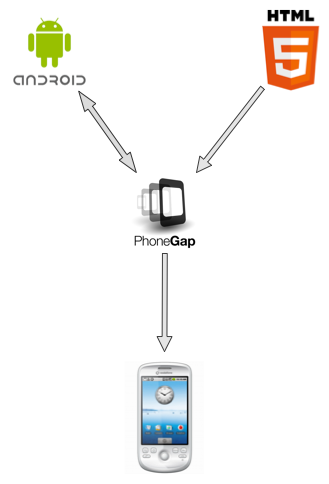
\includegraphics[scale=0.25]{Technologies/phonegapfigure.png}
  \end{center}
  \caption{Building a web application}
\end{wrapfigure}
The basic definition of a web application is: "having no ties to a specific operating system or device". Web applications does not rely on any platform-specific API or SDK. They can be designed to resemble native applications regarding the user interface, and they can be deployed on all major platforms. There are many libraries available for development: JQuery\footnote{http://jquery.com/} and SenchaTouch\footnote{http://www.sencha.com/products/touch} being two. Performance has also increased with the releases of JavaScript engines such as the Google V8\footnote{http://code.google.com/p/v8/}. 

Web applications can consist of web code only, or they can be a hybrid between web applications and native code.  A hybrid application runs the web code, in addition to some parts implemented in native code. This native part can span from simple parts of the user interface, to larger amount of back-end code. What separates a user interface written for web, from a native one, is that the rendering is done by a browser. In native applications, the rendering is done by native graphic components in the device.

The HTML code within web applications can be compiled with a build program. PhoneGap\footnote{www.phonegap.com} is a build API, which maps JavaScript calls to the correct functionalities found in a native SDK. This results in a build file, which is ready to be installed. These actions are depicted in Figure 1, with Android used as an example.

\newpage


\subsubsection{Native Applications}
\label{sec:native}
\begin{wrapfigure}{l}{0.5\textwidth}
  \begin{center}
    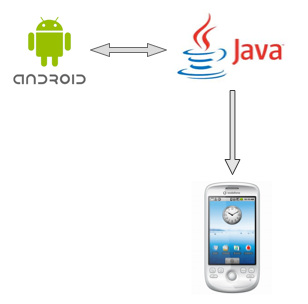
\includegraphics[scale=0.25]{Technologies/javaandroid.png}
  \end{center}
  \caption{Building a native app}
\end{wrapfigure}
Native applications are developed using platform-specific SDKs. Native applications have (through the underlying operating system) direct access to a device's hardware.

The main disadvantage with native development lies in the meaning of the term. As applications are native, they are not portable to other platforms. An application developed for Android cannot be directly run on iOS, or on any other platform. Another disadvantage affecting the TABuss project, is the access to the Google Maps API. The API on the Android platform is accessed through a wrapper, which has several deprecated functionalities. 
Figure 2 depicts the compilation of a native application, with Java as selected programming language, and direct access to the SDK.

\subsubsection {Comparison}
\label{sec:comparison}
Although web applications can perform many of the same functions as native applications, the end result is not always as satisfying.  Web applications (as of today) perform slower than native apps, and large background computing is not supported by build systems (such as PhoneGap\footnote{http://wiki.phonegap.com/w/page/36752779/PhoneGap Plugins}). Graphical Processor Unit(GPU)-acceleration is available for iOS, but not for Android versions older than 3.0\footnote{http://developer.android.com/sdk/android-3.0-highlights.html}, resulting in poorer performance. Still, it is debatable how many applications that actually need performance at a top level to function properly.

Hardware access has earlier been a problem for web, as the possibilities were limited compared to native. Today, provided libraries give access to components such as GPS, camera and compass, and limitations are less visible. However some are noticeable. An example is the usage of maps. For iOS, rendering results are similar to native, while on Android, performance is slower. ''Pinch zoom'' is not possible either. Of the tested applications in section \ref{sec:existingtrondheim}, this was visible in Bartebuss. The map rendering on the iPhone version of Bartebuss, performed much faster than on the Android version. Additionally, problems occurred when turning the screen into/out of landscape mode. This problem has been addressed by MultiBRIS\cite{multibris}.

A fundamental advantage discussed at the Google I/O talks, in favour of native apps, is related to how the web apps can utilise their strength, namely the paradigm:''code once, deploy everywhere''. This is only possible because all technologies based on the web are standardised. The native applications promotor Reto Meier states that: ''Standardised technologies will always trail innovation''. What this means is that while native developers will have direct access to innovative features, web applications may have to wait until a standard is established. Meier continues with the argument that:''If we look at the recent years' rapid development of new technology such as gyroscopes, multi-touch, tablets and so on, all are based on innovations''.

To summarise, both development technologies have advantages and disadvantages. Which one to use depends on the complete context. As mentioned earlier with the argument of Java development being easier than JavaScript, people often chose what they do best. Often, extensive technology research is not possible given strict time limitations, and the learning of a new programming language is not an option. Money also often plays an important part, and the decision can be influenced by the budget. Another interesting aspect is the cost versus profit evaluation. As deployment of an application on multiple platforms may generate more income, it is not an easy decision to make. 

Both TABuss, and Raaum's application, are developed as native applications(for Android). As in many other projects, further development of a system often leads to continuing in the same track. Regarding the map problems discovered in Bartebuss, the question is whether or not a web application for this project actually provides full multi-platform functionality, as its performance clearly is poorer than native applications.

Both of the authors are supporters of native apps, which also affected our choice of technology. We see native applications as ideal for research within mobile development. The end goal for research is seldom mass distribution, but proof-of-concept. This can in our opinion be realised by having the best(native) tools available. 


MultiBRIS\cite{multibris} has chosen to investigate and use web technologies. As a result, the FUIROS project may get a comparison of the two through the development process.

\subsection{Context Awareness}
\label{sec:catechnology}
Context and context awareness have many definitions \cite{Pascoe} \cite{Schilit} \cite{Ryan} \cite{Dey}(1997). In the following sections we first describe location-aware computing, before we review some of the existing definitions of context, and check how TABuss fits into these.
\subsubsection{Location-aware Computing}
Smartphones today are pervasive\footnote{http://en.wikipedia.org/wiki/Ubiquitous\_computing} and personal. This means that they are almost always turned on, and they are customised to each user. Raento, Oulasvirta, Petit and Toivonen(2005) claimed that because of this, smartphones are well suited for context-aware applications\cite{raento}.

Hazas,Scott and Krumm(2002) stated that: \emph{context awareness is at the core of location-aware computing\cite{hazas}}. Location-aware systems use the user's location in functionalities, through a location-sensing technology. A location-sensing technology is not restricted to GPS or WiFi, but also includes Radio frequency identification(RFID)\footnote{http://no.wikipedia.org/wiki/Radio\_Frequency\_Identification}. RFID tags have a short transmission range compared to GPS and WiFi. An example of RFID use in a context aware application is to place tags in door entries, and track passing people.

A domain of context awareness is in tourist guide applications. Wang, S\o rensen, Brede, Servold and Gimre, in 2005, developed the context aware \emph{Nidaros Framework}\cite{wang}. Using this framework they implemented a tour guide for the Nidaros Cathedral\footnote{http://en.wikipedia.org/wiki/Nidaros\_Cathedral}, which uses the user's location to display zones and nearby objects.

Because of the arguments stated by Raento, Oulasvirta, Petit and Toivonen, we claim that the domain of bus route information systems is well suited for context awareness. Such systems should be able to monitor the user's behaviour through sensor input, and use this data to provide route suggestions or other information.

\subsubsection{Definitions}
Pascoe (1998) defined context to be ``a subset of physical and conceptual states of interest to a particular entity''\cite{Pascoe}, where the importance of the involved states had to be determined. An example of an entity could be a person.

Schilit and Theimer(1994)  defined context by three factors: location, descriptions of people in the immediate surroundings and objects with the changes these objects go through\cite{Schilit}. This is a broad definition, with essential criteria needed to be fulfilled, in order to be classified as context.

Ryan et al. (1997)  defined context as the user's location, environment, identity and time\cite{Ryan}. Context is generalised by including a number of physical and logical attributes, assumed to affect the user's environment. The definition has similarities to Schilit and Theimer's 1994 proposal, in terms of important factors. However, Ryan et al.(1997) introduces time as an additional factor.

Dey (1997) defined context in a more general formulation, and not by enumerating a list of factors needed to be matched, in order to be called context: ''context is any information that can be used to characterise the situation of an entity. An entity is a person, place or object that is considered relevant to the interaction between a user and an application, including the user and application themselves''\cite{Dey}. This formulation simplifies declaring functionalities and theories as context. If any part of information can describe or help the user at a given time, it can be called context.

Our project uses \emph{context} and \emph{context awareness} in two different ways. The former context uses the user's location, while the latter context introduces time and destination as additional factors. Schilit and Theimer's(1994) and Ryan et al.'s(1997) definitions, would consider the limited and changing factors not to be adaptable to our purpose, as this would lead to forcing our factors into their definitions.

Pascoe's(1998) definition cannot be used, because of the lack of modularity. If adding additional factors to determine context, their importance would have to be determined: this is difficult, as situations change(what is rated as an important factor in one setting, might be less important in another).

Dey's(1997) definition is the one best suited for our project. This is because of its generality, which defines a factor to be a part of the context, as long as it concerns the user. It also allows for context to be either implicit or explicit. This means that context information is both provided by the user and automatically detected by the system. Dey also defines ''context awareness'' as the system's response to changed context. It does not determine whether the system should initiate an action automatically or not(in our project, this fits). In a practical example from TABuss: the system should not automatically start downloading the real-time data for one or more stops, only because the user has changed his/her location. But in an intelligent application, it is still an advantage to have the option to do so.

As mentioned earlier, context and context awareness are used in two different ways. Context is used during the general location tracking of the user, and subsequent loading of nearby bus stops. This happens dynamically as the user moves and can be seen on the map while moving: clickable bus stop icons are added or removed as the user changes his/her location. This is an example of implicit context: the user does not provide the location information manually(location is automatically detected and tracked by the system). However, a location technology such as GPS, WiFi or 3G must be enabled.

The second way, which uses more factors(e.g. time and day), is described in Section \ref{sec:contextawareness}.






